\begin{frame}[c]
    \begin{columns}[onlytextwidth]
    \begin{column}{0.55\textwidth}
    \textbf{IceCube Neutrino Observatory}
        \begin{itemize}
            \item PROPOSAL used in the IceCube simulation chain
            \begin{itemize}
                \item[$\rightarrow$] Simulation of muons and taus in ice
                \item[$\rightarrow$] PROPOSAL provides the energy losses along the particle track
                \item[$\rightarrow$] Energy losses are further processed by other tools to simulate Cherenkov photons
            \end{itemize}
        \end{itemize}
    \end{column}
        \begin{column}{0.45\textwidth}
            \begin{figure}
                \centering
                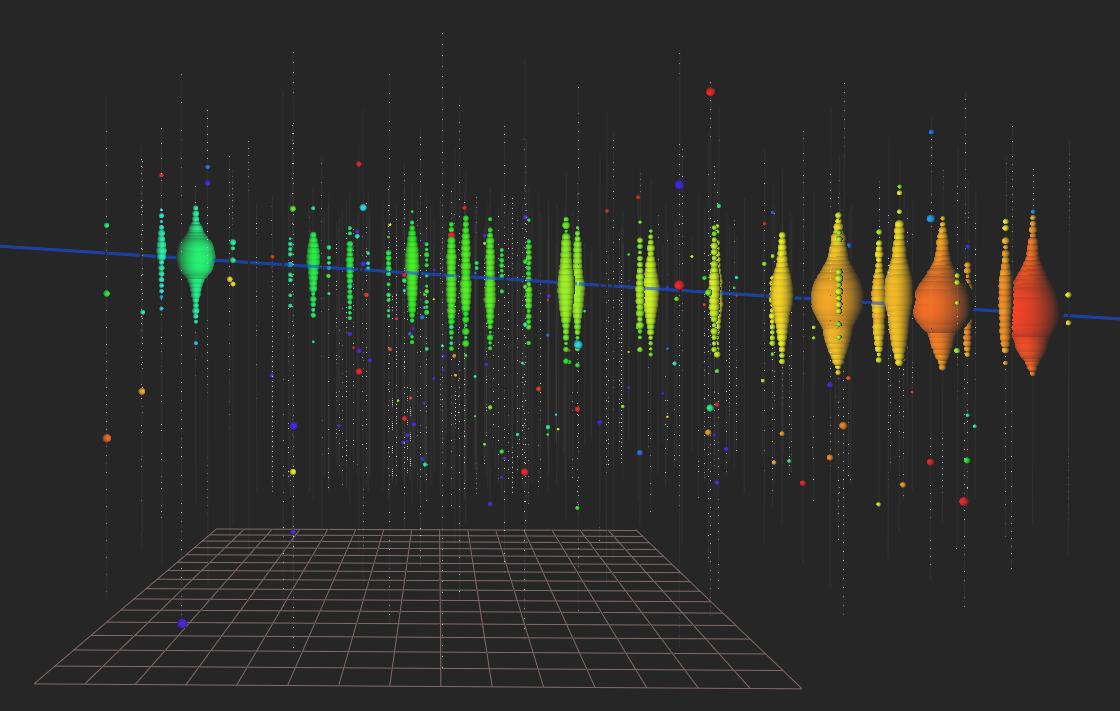
\includegraphics[width=0.9\textwidth]{images/Track.png}
                \credit{IceCube Collaboration}
            \end{figure}
        \end{column}
    \end{columns}
\end{frame}


\begin{frame}[c]
    \begin{columns}[onlytextwidth]
    \begin{column}{0.6\textwidth}
    \textbf{CORSIKA 8}
        \begin{itemize}
            \item PROPOSAL used in CORSIKA~8 as an electromagnetic shower model
            \begin{itemize}
                \item[$\rightarrow$] CORSIKA uses propagation steps, provided by PROPOSAL modules
            \end{itemize}
        \end{itemize}

        \hspace{10pt} $\Rightarrow$ Talks dedicated to CORSIKA~8: \href{https://www.dpg-verhandlungen.de/year/2022/conference/heidelberg/part/t/session/47/contribution/8}{\textbf{T47.8}}, \href{https://www.dpg-verhandlungen.de/year/2022/conference/heidelberg/part/t/session/72/contribution/5}{\textbf{T72.5}}, \href{https://www.dpg-verhandlungen.de/year/2022/conference/heidelberg/part/t/session/72/contribution/7}{\textbf{T72.7}}, \href{https://www.dpg-verhandlungen.de/year/2022/conference/heidelberg/part/akpik/session/1/contribution/7}{\textbf{AKPIK1.7}}

    \end{column}
        \begin{column}{0.4\textwidth}
            \begin{figure}
                \centering
                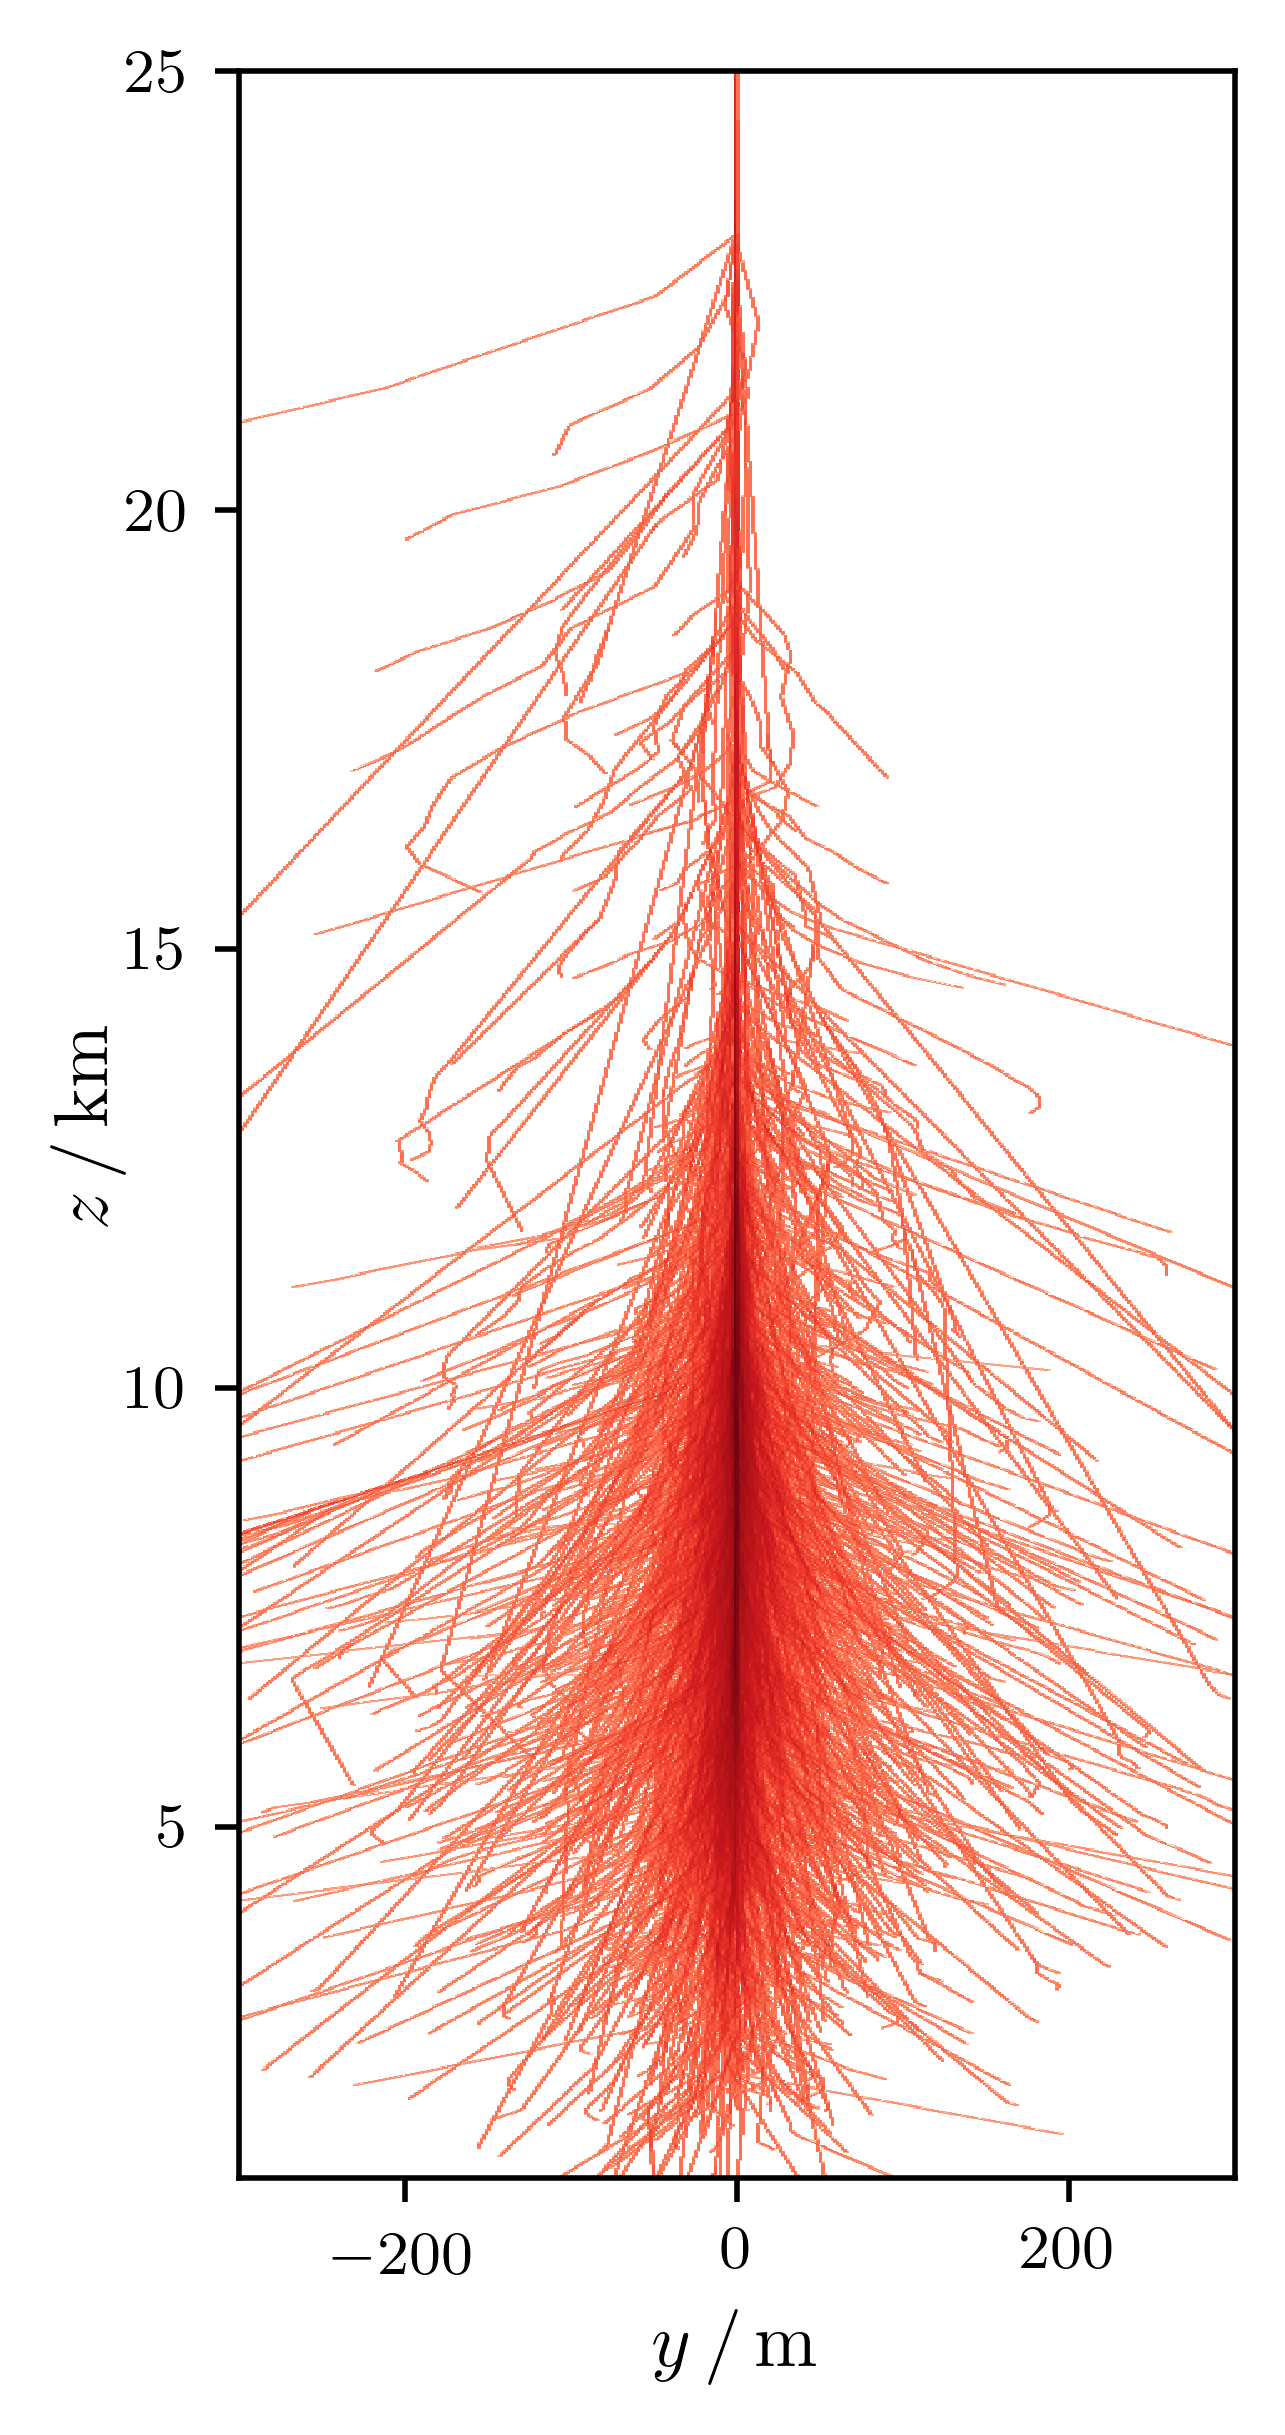
\includegraphics[width=0.6\textwidth]{plots/shower.png}
                \caption*{\SI{1}{\tera\electronvolt} $e^-$ shower simulated with CORSIKA 8}
            \end{figure}
        \end{column}
    \end{columns}
\end{frame}

